\chapter{\LaTeX{} 畫圖}
畫圖雖然有 ipe, inkscape 等工具,不過直接在紙上畫會更精準一點,所以
使用 macro 畫圖雖然痛苦但也精準有趣,只不過要多記一些東西。

\section{picture}
picture 是最基本的畫圖 package,主要用 
\begin{itemize}
  \item unitlength 設定畫線單位
  \item put(x, y)\{object\} 畫預設物件,像直線,圓,方塊等等。
  \item multiput(x, y)(dx,dy)\{n\}\{object\} 畫 n 個複製物件
  \item qbezier(x1, y1)(x2, y2)(x3, y3) 貝茲曲線畫彎線,3 個控制點。
\end{itemize}
命令來畫物件,x,y 是相對於畫線單位的數字長度,multiput 的 dx, dy 是
delta 的意思,表示從 x,y 長出多少後面物件,然後複製 n 個。
預設\href{https://latexref.xyz/picture.html}{物件}有 line, circle ...等等
\\\\
基本設定為
\begin{verbatim}
\setlength{\unitlength}{1.2cm}
\begin{picture}(x, y)(x0, y0)
...
\end{picture}
\end{verbatim}
x,y 是畫圖方塊畫布,x0,y0 是相對於畫布的座標系統原點,這通常沒有用。例如
\begin{verbatim}
\setlength{\unitlength}{1cm}
  \begin{picture}(5,5)
    \put(0,0){\line(0,1){3}}
    \put(-1,0){\line(1,1){4}}
    \put(0,2){\line(1,1){1}}
    \put(1,0){\line(1,2){2}}
\end{picture}
\end{verbatim}
上面定義了一張5x5公分的畫布,他會根據所有 input 自動調整座標系的最大最小
範圍。畫了四根線, 分別從 (0,0) (-1,0) (0,2) (1,0) 畫出,然後方向向量是
根據 put 的座標的相對座標長一個長度。所以(-1,0) 開始往相對他的 (1,1),就是
原本座標的 (0,1) 方向,走 4 個長度。
\begin{center}
\setlength{\unitlength}{1cm}
  \begin{picture}(5,5)
    \put(0,0){\line(0,1){3}}
    \put(-1,0){\line(1,1){4}}
    \put(0,2){\line(1,1){1}}
    \put(1,0){\line(1,2){2}}
\end{picture}
\end{center}
例子就只能多看,就會了
\begin{verbatim}
\setlength{\unitlength}{1cm}
\begin{picture}(6,6)(-3,-3)
\put(-1.5,0){\vector(1,0){3}}
\put(2.7,-0.1){$\chi$}
\put(0,-1.5){\vector(0,1){3}}
\multiput(-2.5,1)(0.4,0){13}
{\line(1,0){0.2}}
\multiput(-2.5,-1)(0.4,0){13}
{\line(1,0){0.2}}
\put(0.2,1.4)
{$\beta=v/c=\tanh\chi$}
\qbezier(0,0)(0.8853,0.8853)
(2,0.9640)
\qbezier(0,0)(-0.8853,-0.8853)
(-2,-0.9640)
\put(-3,-2){\circle*{0.2}}
\end{picture}
\end{verbatim}
\begin{center}
\setlength{\unitlength}{1cm}
\begin{picture}(6,6)(-3,-3)
\put(-1.5,0){\vector(1,0){3}}
\put(2.7,-0.1){$\chi$}
\put(0,-1.5){\vector(0,1){3}}
\multiput(-2.5,1)(0.4,0){13}
{\line(1,0){0.2}}
\multiput(-2.5,-1)(0.4,0){13}
{\line(1,0){0.2}}
\put(0.2,1.4)
{$\beta=v/c=\tanh\chi$}
\qbezier(0,0)(0.8853,0.8853)
(2,0.9640)
\qbezier(0,0)(-0.8853,-0.8853)
(-2,-0.9640)
\put(-3,-2){\circle*{0.2}}
\end{picture}
\end{center}
circle* 表示是個填滿黑色的實心圓。

\section{pgfplots}
簡單的 pgfplots 使用 pgfplots package 跟 pgfplotsset 來設定真實大小, 是
很好畫 x-y 圖的工具。 pgfplots 是基於 tikz 的 plot 系統,能夠快速畫出座標
系統,能做 symbolic 運算畫圖, 也能引進實驗數據,畫出 X-Y 圖。
內定 texlive 是沒有裝,要自己 tlmgr install pgfplots,
\begin{verbatim}
\usepackage{pgfplots}
\pgfplotsset{compat=1.18,width=10cm}

  \begin{tikzpicture}

  \begin{axis}[xmin=-2,xmax=2,ymin=-2,ymax=2]
  \addplot[color=red,dashed,mark=*,samples=50]{x^2};
  \end{axis}

  \end{tikzpicture}
\end{verbatim}
\begin{center}
\begin{tikzpicture}
  \begin{axis}[xmin=-2,xmax=2,ymin=-2,ymax=2]
  \addplot[color=red,dashed,mark=*,samples=50]{x^2};
  \end{axis}
\end{tikzpicture}
\end{center}
這個例子畫了$x^2$,用了 50 個取樣點,取樣點越多就越平滑。
主要是 tikzpicture 跟 axis 這兩個 environment,然後 axis 環境的選項中括號,還
必須順序在後面, 最後要注意的是 tikzpicture 的命令是以分號 semiclone 結束
\\\\
pgfplot 還提供很方便的外部 data X-Y 圖,假設有兩個檔案 data1.txt 跟 data2.txt
\begin{verbatim}
data1.txt           data2.txt

1 10                1 30
2 20                2 70
3 40                3 100
4 80                4 170
5 160               5 280
\end{verbatim}
然後只要用 table 引進檔名,就會自己畫出 X-Y 圖
\begin{verbatim}
  \begin{tikzpicture}
    \begin{axis}[
      title={my x-y},
      xlabel={$x-axis$},
      ylabel={$y-axis$},
      legend entries={data1,data2},
      legend pos={south east}
    ]
    \addplot table {data1.txt};
    \addplot table {data2.txt};
    \end{axis}
  \end{tikzpicture}
\end{verbatim}
  \begin{center}
  \begin{tikzpicture}
    \begin{axis}[
      title={my x-y},
      xlabel={$x-axis$},
      ylabel={$y-axis$},
      legend entries={data1,data2},
      legend pos={south east}
    ]
    \addplot table {data1.txt};
    \addplot table {data2.txt};
    \end{axis}
  \end{tikzpicture}
  \end{center}
  其中還用上了 X-Y 圖的圖例標籤 legend,與X-Y軸的 label 文字。legend 的位置,
  可以從 pos 指定,south east 表示放在東南邊。
  而除了大軸用的 xlabel, ylabel 外, 座標系統的標注可以用 xticklabel,
  yticklabel 來使用
\begin{verbatim}
  \begin{tikzpicture}

  \begin{axis}[
    xmin=0,xmax=2*pi,ymin=-2,ymax=2,
    axis line=middle,
    xticklabels={$0$,$\frac{\pi}{2}$,$\pi$,$\frac{3}{2}\pi$,$2\pi$},
    xticklabel style={anchor=south west},
    xtick={0,pi/2,pi,3*pi/2,2*pi},
    xmajorgrids=true,
    grid style=dashed
  ]
  \addplot[domain=0:2*pi,color=blue]{sin(deg{x})} node[right,pos=0.3]{$f(x) = sin(x)$};

  \end{axis}

  \end{tikzpicture}
\end{verbatim}

\begin{center}
\begin{tikzpicture}

  \begin{axis}[
    xmin=0,xmax=2*pi,ymin=-2,ymax=2,
    axis lines=middle,
    xticklabels={$0$,$\frac{\pi}{2}$,$\pi$,$\frac{3}{2}\pi$,$2\pi$},
    xticklabel style={anchor=south west},
    xtick={0,pi/2,pi,3*pi/2,2*pi},
    xmajorgrids=true,
    grid style=dashed
  ]
  \addplot[domain=0:2*pi,color=blue]{sin(deg(x))} node[right,pos=0.3]{$f(x) = sin(x)$};
  \end{axis}

\end{tikzpicture}
\end{center}
使用很多選項標注文字,在 plot 裡面標注文字用 node,pos=1 表示在 sin 圖
的 100\%處標上文字,可以用 0 到 1 表示百分比。xticklabel 的 style 是標注文字
的位置,anchor 在西南,表示 xticklabel 在 x 軸的東北。

\section{TIKZ}
pgfplots 是 based 在 tikz 之上,所以他很方便,但我們也可以用 tikz 畫圖,相比較
更基本的 picture ,他有更多的選項與搭配的 library, 像樂譜,下棋,甚至還有像鴨
子, tikzducks,library 都要額外自己裝 package,但用 tlmgr 裝很快就裝起來。
\\\\
當使用原始的 tikzpicture 時,則要用 draw 這個命令去畫圖,\LaTeX{} 畫圖,都有
個座標系統,大小會自動根據所有輸入數值,找到最大最小設定, tikz 可以給座標名字
,將來好方便使用,$x-y$ 座標多以 (x,y) 表現 ,$r-\theta$ 座標則以
($\theta$:$r$) 表示, 內定值是點, 使用內定的單位就是 pt 約等於 0.35mm ,
但也可以用 (1cm,2cm) 這種方法設定, (start-angle:end-angle:radius) 表示畫弧線,
start 跟 end angle 是從正水平 x 軸逆時針開始量測。 基本命令為
\begin{itemize}
  \item coordinate 設定不同座標點成名字,畫圖命令可以用,其實就是裡面代換。
  \item draw 一個命令給不同參數畫直線,貝茲曲線等等,但最抽象物件為 node。
  \item draw node 物件可以有 node 命令直接標注文字
\end{itemize}
\begin{verbatim}
\begin{tikzpicture}
  \coordinate (A) at (2,3);

  \draw (-2,0) -- (2,0);
  \filldraw [gray] (0,0) circle (2pt);
  \draw (-2,-2) .. controls (0,0) .. (2,-2);
  \draw (-2,2) .. controls (-1,0) and (1,0) .. (2,2);

  \draw (A) arc (30:90:2);
  \draw (A) node {在 A node 物件};
  \draw (-1,-1) node { 我是 node 物件};
  \node at (1,1) { 相對座標系 1,1 };
\end{tickpicture}
\end{verbatim}
\begin{center}
\begin{tikzpicture}
  \coordinate (A) at (2,3);
  \draw (-2,0) -- (2,0);
  \filldraw [gray] (0,0) circle (2pt);
  \draw (-2,-2) .. controls (0,0) .. (2,-2);
  \draw (-2,2) .. controls (-1,0) and (1,0) .. (2,2);
  \draw (A) arc (30:90:2);
  \draw (A) node {在 A node 物件};
  \draw (-1,-1) node { 我是 node 物件};
  \node at (1,1) { 相對座標系 1,1 };
\end{tikzpicture}
\end{center}
上面畫線用 \verb=--=  ,畫貝茲曲線用 \verb=..=,
定義一個新名字 A 等於是 (2,3) 這個點,用 node 在座標系上標上想要文字。
字串中心點才是 node 設的座標。
\\\\
例子
\begin{verbatim}
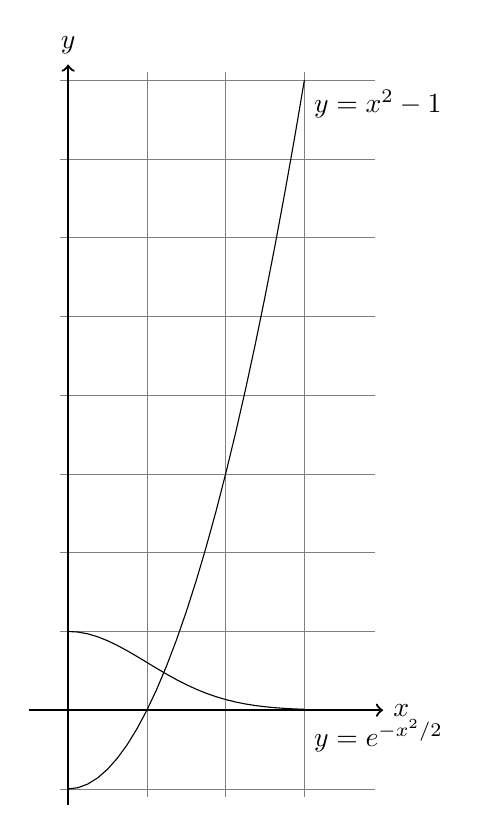
\begin{tikzpicture}
\draw[very thin,color=gray] (-0.1,-1.1) grid (3.9,8.1);
\draw[->,thick] (-0.5,0) -- (4,0) node[right] {$x$};
\draw[->,thick] (0,-1.2) -- (0,8.2) node[above] {$y$};

\draw[domain=0:3] plot (\x,{\x*\x-1}) node[below right] {$y = x^2-1$};
\draw[domain=0:3] plot (\x,{exp(-\x*\x/2)}) node[below right] {$y = e^{-x^2/2}$};
\end{tikzpicture}
\end{verbatim}

\begin{center}
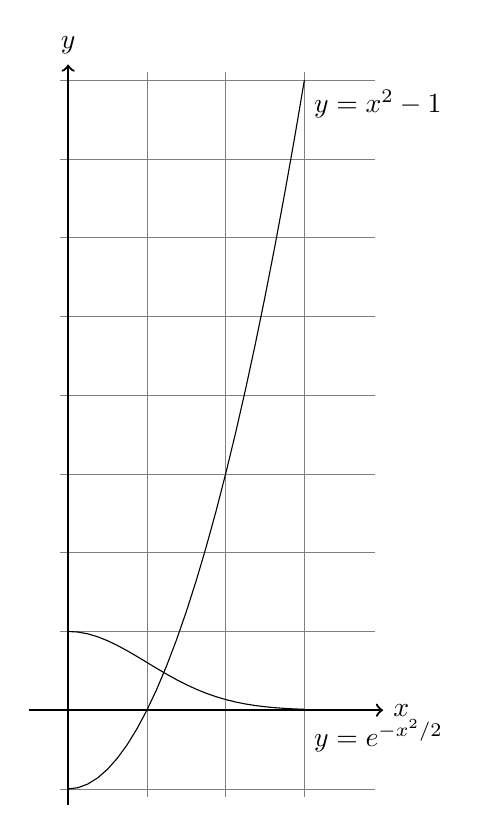
\begin{tikzpicture}
\draw[very thin,color=gray] (-0.1,-1.1) grid (3.9,8.1);
\draw[->,thick] (-0.5,0) -- (4,0) node[right] {$x$};
\draw[->,thick] (0,-1.2) -- (0,8.2) node[above] {$y$};

\draw[domain=0:3] plot (\x,{\x*\x-1}) node[below right] {$y = x^2-1$};
\draw[domain=0:3] plot (\x,{exp(-\x*\x/2)}) node[below right] {$y = e^{-x^2/2}$};
\end{tikzpicture}
\end{center}
重點是
\begin{itemize}
  \item 一樣用中括號設定參數,用 ( ) 設定起始點,終點
  \item 畫格子 grid,除了 grid 還有之前看到的 circle, rectangle...。
  \item node 寫文字, 擺設位置設定在起始點的 below, above, right, left,
    在 pgfplots 裡面用east, south, west, north 東南西北表示。
  \item 用 \verb=->= 畫箭頭
  \item 用 color 畫顏色
  \item 指定線粗細用 thin, thick ...
  \item plot 畫 symbolic 運算
  \item domain 設定 symbolic 運算範圍
\end{itemize}
顏色與粗細設定
\begin{itemize}
  \item black, red, green, blue, cyan, magenta, ...
  \item ultra thin, very thin, thin 三種 thin
  \item ultra thick, very thick, thick 三種 thick
\end{itemize}
\begin{center}
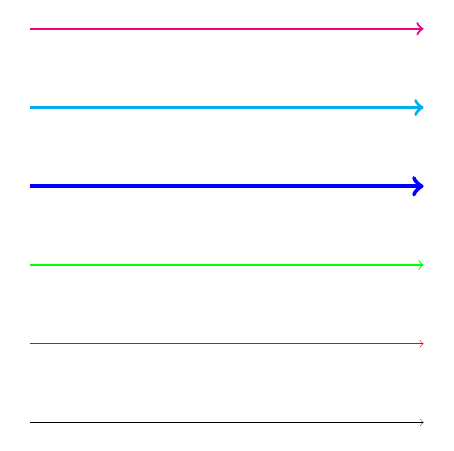
\begin{tikzpicture}
\draw[->,ultra thin, color=black] (0,1) -- (5,1);
\draw[->,very thin,color=red] (0,2) -- (5,2);
\draw[->,thin,color=green] (0,3) -- (5,3);
\draw[->,ultra thick,color=blue] (0,4) -- (5,4);
\draw[->,very thick,color=cyan] (0,5) -- (5,5);
\draw[->,thick,color=magenta] (0,6) -- (5,6);
\end{tikzpicture}
\end{center}
最後 tikzpicture 有很多 library 可以套用,只要用 usetikzlibrary 引用
,例如 patterns 跟 snakes
\begin{verbatim}
\usetikzlibrary{patterns,snakes}

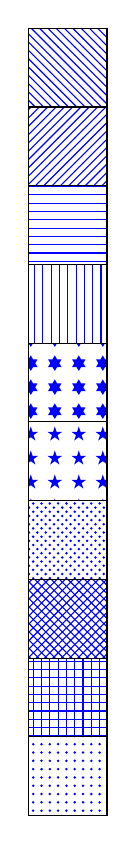
\begin{tikzpicture}
\draw[pattern=dots, pattern color=blue] (0,0) rectangle ++(1,1);
\draw[pattern=grid, pattern color=blue] (0,1) rectangle ++(1,1);
\draw[pattern=crosshatch, pattern color=blue] (0,2) rectangle ++(1,1);
\draw[pattern=crosshatch dots, pattern color=blue] (0,3) rectangle ++(1,1);
\draw[pattern=fivepointed stars, pattern color=blue] (0,4) rectangle ++(1,1);
\draw[pattern=sixpointed stars, pattern color=blue] (0,5) rectangle ++(1,1);
\draw[pattern=vertical lines, pattern color=blue] (0,6) rectangle ++(1,1);
\draw[pattern=horizontal lines, pattern color=blue] (0,7) rectangle ++(1,1);
\draw[pattern=north east lines, pattern color=blue] (0,8) rectangle ++(1,1);
\draw[pattern=north west lines, pattern color=blue] (0,9) rectangle ++(1,1);
\end{tikzpicture}
\end{verbatim}
\begin{center}
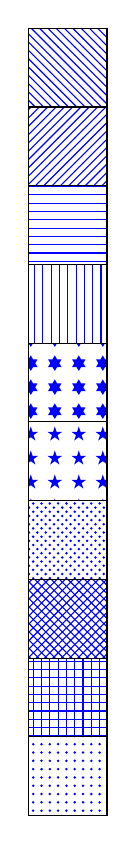
\begin{tikzpicture}
\draw[pattern=dots, pattern color=blue] (0,0) rectangle ++(1,1);
\draw[pattern=grid, pattern color=blue] (0,1) rectangle ++(1,1);
\draw[pattern=crosshatch, pattern color=blue] (0,2) rectangle ++(1,1);
\draw[pattern=crosshatch dots, pattern color=blue] (0,3) rectangle ++(1,1);
\draw[pattern=fivepointed stars, pattern color=blue] (0,4) rectangle ++(1,1);
\draw[pattern=sixpointed stars, pattern color=blue] (0,5) rectangle ++(1,1);
\draw[pattern=vertical lines, pattern color=blue] (0,6) rectangle ++(1,1);
\draw[pattern=horizontal lines, pattern color=blue] (0,7) rectangle ++(1,1);
\draw[pattern=north east lines, pattern color=blue] (0,8) rectangle ++(1,1);
\draw[pattern=north west lines, pattern color=blue] (0,9) rectangle ++(1,1);
\end{tikzpicture}
\end{center}
snakes
\begin{verbatim}
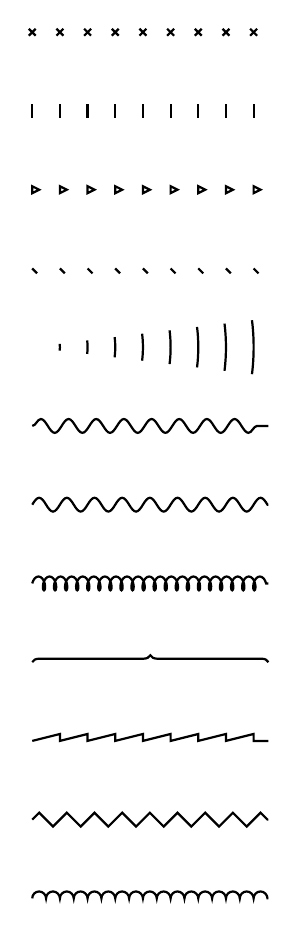
\begin{tikzpicture}[thick]
\draw[snake=bumps] (0,0) -- (3,0);
\draw[snake=zigzag] (0,1)-- (3,1);
\draw[snake=saw] (0,2) -- (3,2);
\draw[snake=brace] (0,3)-- (3,3);
\draw[snake=coil,segment length=4pt] (0,4)-- (3,4);
\draw[snake=coil,segment aspect=0] (0,5) -- (3,5);
\draw[snake=snake] (0,6) -- (3,6);
\draw[snake=expanding waves,segment angle=7] (0,7)-- (3,7);
\draw[snake=border,segment angle=-45] (0,8) -- (3,8);
\draw[snake=triangles] (0,9) -- (3,9);
\draw[snake=ticks] (0,10) -- (3,10);
\draw[snake=crosses] (0,11) -- (3,11);
\end{tikzpicture}
\end{verbatim}
\begin{center}
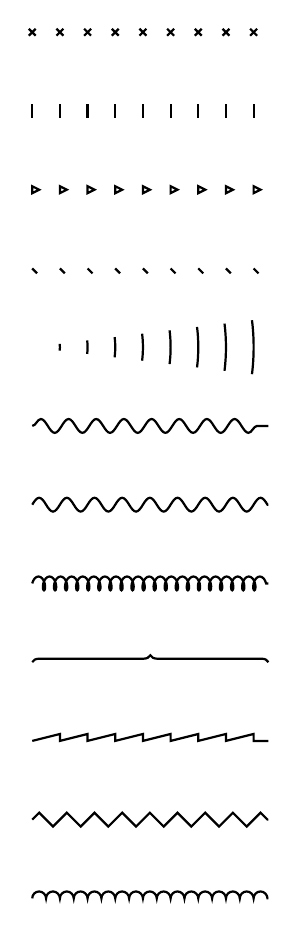
\begin{tikzpicture}[thick]
\draw[snake=bumps] (0,0) -- (3,0);
\draw[snake=zigzag] (0,1)-- (3,1);
\draw[snake=saw] (0,2) -- (3,2);
\draw[snake=brace] (0,3)-- (3,3);
\draw[snake=coil,segment length=4pt] (0,4)-- (3,4);
\draw[snake=coil,segment aspect=0] (0,5) -- (3,5);
\draw[snake=snake] (0,6) -- (3,6);
\draw[snake=expanding waves,segment angle=7] (0,7)-- (3,7);
\draw[snake=border,segment angle=-45] (0,8) -- (3,8);
\draw[snake=triangles] (0,9) -- (3,9);
\draw[snake=ticks] (0,10) -- (3,10);
\draw[snake=crosses] (0,11) -- (3,11);
\end{tikzpicture}
\end{center}
鴨子
\begin{verbatim}
\usetikzlibrary{ducks}


\begin{tikzpicture}
  \draw (0,0) pic[
    duck/water=green,
    duck/alien,
    ] {duck};
  \draw (4,0) pic[
    scale=1.4,
    ] {duck};
\end{tikzpicture}
\end{verbatim}
\begin{center}

\begin{tikzpicture}
  \draw (0,0) pic[
    duck/water=green,
    duck/alien,
    ] {duck};
  \draw (4,0) pic[
    scale=1.4,
    ] {duck};
\end{tikzpicture}
\end{center}
這些工具所畫圖都能跟之前插圖用的 figure, wrapfig 共用,也能用上索引 caption。
\\\\
其實還有很多其他有趣的畫圖工具,有的畫工程圖或 x-y 圖也很漂亮,基本上三種繪圖
工具都非常多設定,所以最後還是要 google 看人家的範例改成自己想要的,無論什麼圖
,大致都能快速精準畫出。
